% ========各チャプタ用テンプレート (update: 2023/11/29)========
%  チャプタごとにファイルを作成して利用することを想定．

% このファイル単体でPDFに変換する際にはファイルをまたぐ相互参照は「??」となるので注意(警告なのでPDFは生成される， 表示確認用を想定)．
% いずれの場合も章番号は1からになる(main.texでは正しく割り振られる)

% このファイルのプリアンブルに記述したパッケージはmain.texでは反映されないので注意．

% このファイルを単体で実行するときも， main.texのプリアンブルが読み込まれるようになっているので，
% 設定は main.texのプリアンブル or mysettings.styに記述すれば良い(後者を推奨)．

\documentclass[main]{subfiles}

% ここのプリアンブルには何も書かないこと(main.texで反映されないので)

\begin{document}

\chapter{このテンプレートについて}

\cite{2017latex2ε美文書作成入門}を参考に作成した．

\section{動作環境}

このテンプレートはTeXLive 2022を用い，macOSで動作確認をしている．
確認済みの\TeX エンジンは以下の通り：
\begin{itemize}
  \item p\LaTeX
  \item up\LaTeX
  \item Lua\LaTeX
\end{itemize}

ここに挙げた\TeX エンジンであれば，\textbf{同じソースファイル\texttt{(main.tex)}で動作する}．
ただし，up\LaTeX の利用を推奨する．
Lua\LaTeX については出力が上記2つと異なる部分があるが，とりあえずPDF生成ができたくらいのクオリティ
でバグがまだまだ有りそうなので，普段Lua\LaTeX を利用していてバグ修正ができる人の利用に留めてほしい．
\footnote{筆者はup\LaTeX を使っているので詳しい人はいい感じに修正してくれると助かります．}．

\section{利用方法}

このテンプレートは，章ごとに\TeX ファイルを分割して利用することを想定して作成している．
分割したファイルを集約して1つの文書として生成するためのメインファイルが\texttt{main.tex}である．

メインファイルの文量が多くなり，実行に時間がかかりすぎるようになってしまった場合には，
分割した\TeX ファイル単体でも実行することが可能である．
ただし，その場合は章のナンバリングが1から始まり，章をまたぐ相互参照が適用されなくなる．
サクッと出力を確認するための機能である．

\subsection{メインファイルの記述法}

メインファイルでは，プリアンブル\footnote{\texttt{\textbackslash documentclass}から\texttt{\textbackslash begin\{document\}}の間}
にタイトルや氏名などの論文情報を記述する．
詳細な記述方法はソースファイルを見れば理解できるだろう．

\TeX ファイルを追加する場合は\verb|\subfile|コマンドを利用する．
例えば，\verb|sample.tex|を追加したい場合は\verb|\subfile{sample}|のように
拡張子なしでファイル名を記載すれば良い．

\subsection{分割したい\TeX ファイルの記述法}

分割したい\TeX ファイルのドキュメントクラスは以下のように記述する：
\begin{verbatim}
      \documentclass[main]{subfiles}
\end{verbatim}
これにより，メインファイルのドキュメントクラス・プリアンブルと同一の
内容を読み込むことができる．
そのため，使いたいパッケージや自作コマンドについてはメインファイルのプログラム or \texttt{mysettings.sty}(後述)に記載することを推奨する．
それ以外の\TeX ファイルのプリアンブルに記述した内容は，メインファイルの実行時に読み込まれないのでエラーの原因となり得る．

\subsection{スタイルファイル}

このテンプレートで用いている独自のスタイルファイルには
\texttt{tuats.sty}と\texttt{mysettings.sty}の2種類がある．

\paragraph{\texttt{tuats.sty}}

このファイルでは，共通ページのレイアウト設定や独自の変数の定義を行っている．
\TeX に詳しくない人はあまり触らないほうが安心できるだろう．

\paragraph{\texttt{mysettings.sty}}

このファイルでは，パッケージの読み込みやフォント設定などのユーザの好みで書き換えそうな設定を行っている
\footnote{ただ，複数の\TeX エンジンに対応させるようにしようと修正しているうちにファイルが煩雑になってしまったように思えるので，いずれは綺麗にしたい...}．
何か追加したい場合は，このファイルの下側に書き加えると良い．

\section{図表の表示}

相互参照のナンバリングは\textbf{章ごと}に行われる(\tabref{tab:example_table}, \figref{fig:example_image})．
表目次と図目次にも自動で追加される．

\begin{table}[H]
  \centering
  \caption{適当な表}
  \label{tab:example_table}
  \begin{tabular}{c|c|c}
    \hline
    a & b & c \\
    d & e & f \\
    \hline
  \end{tabular}
\end{table}

\begin{figure}[htbp]
  \centering
  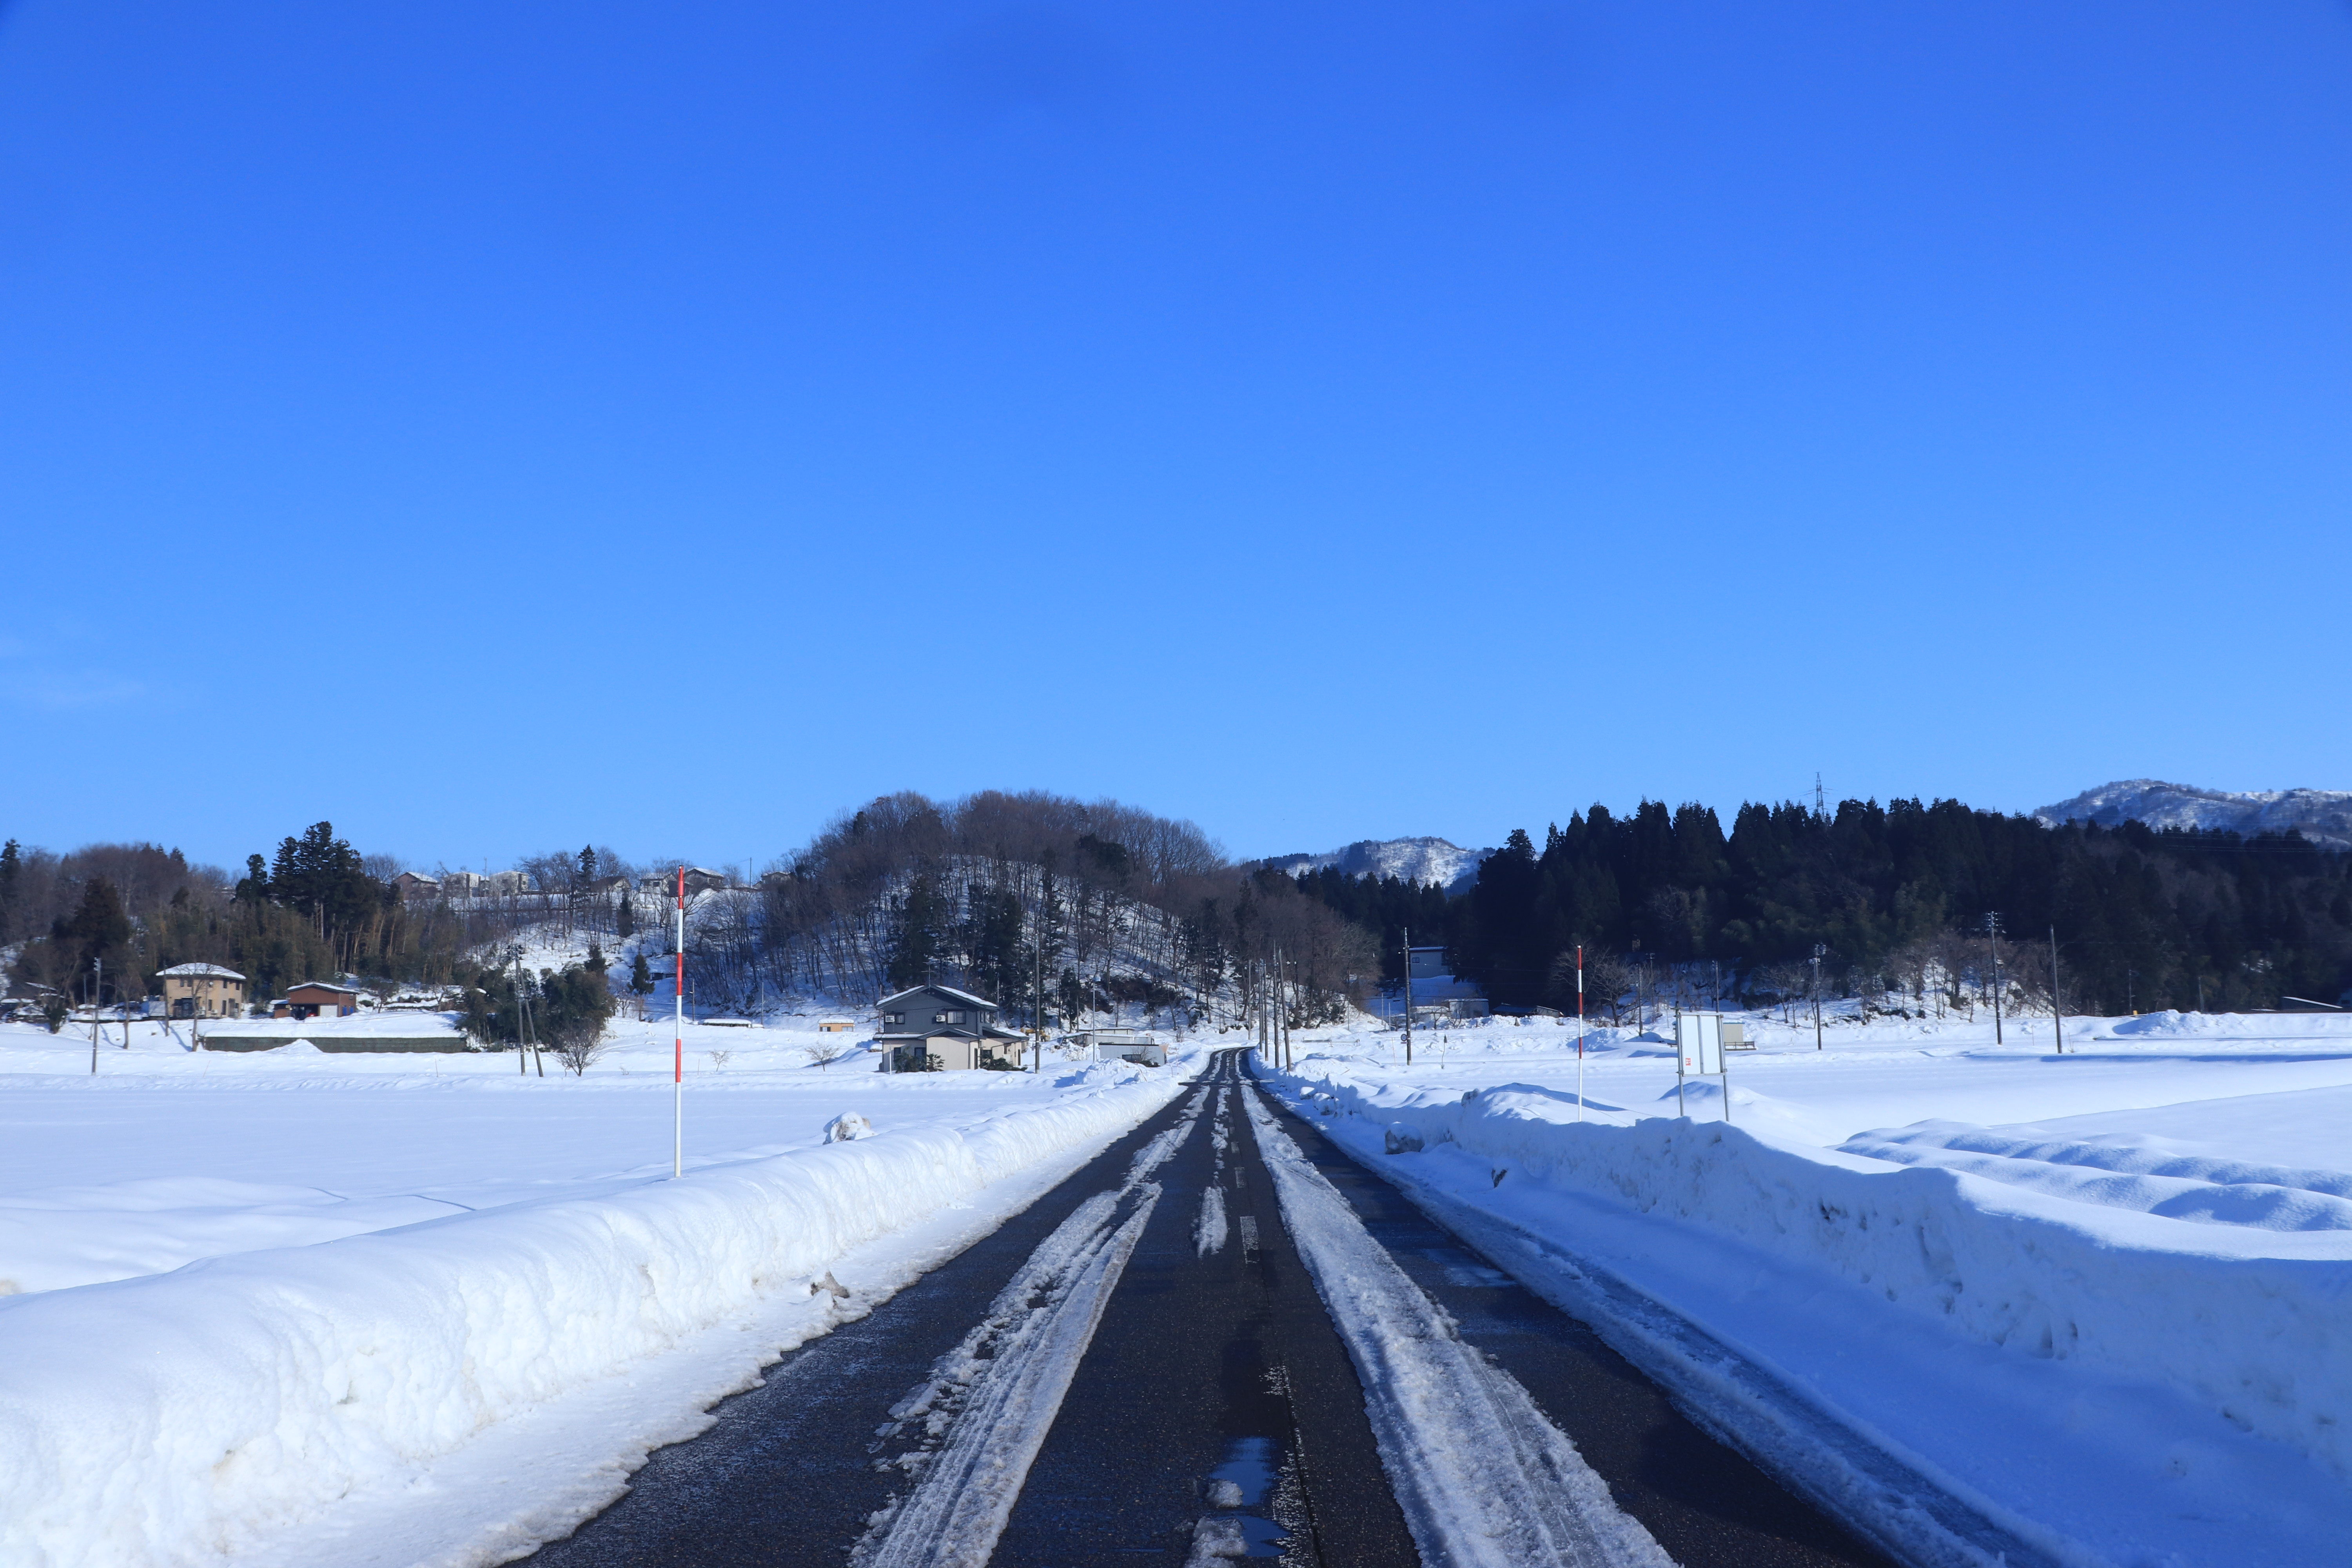
\includegraphics[width=0.7\linewidth]{figures/nagaoka.JPG}
  \caption{真冬の新潟県長岡市(2021年1月21日)}
  \label{fig:example_image}
\end{figure}

なお，図表の相互参照については効率よく記述するためのコマンドを定義しておいてある．
例えば，図の相互参照の場合は\verb|\figref{fig:sample1}|，表の場合は\verb|\tabref{tab:sample2}|
\footnote{表を\texttt{tbl}と書く派閥向けに\texttt{\textbackslash tblref}も作成してある．}
のように記述すれば，「\tabref{tab:example_table}」, 「\figref{fig:example_image}」
のような形式で表示される．

他にも，式の参照を行う\verb|\equref|，章の参照を行う\verb|\chapref|，節の参照を行う\verb|\secref|
，項の参照を行う\verb|\subsecref|も作成してある．

\section{数式表示}

数式については左寄せにしてある．
中央寄せにしたい場合はドキュメントクラスの\texttt{fleqn}を削除すれば良い．
\begin{equation}
  ax^2 + bx + c = 0
\end{equation}

\section{最後に}

このテンプレートは，筆者が高専時代に作成したテンプレートと藤田桂英研究室の先輩が作成してくださったスタイルファイル
の良いところをマージして作成したものである．
そのため，想定しないバグが隠れている可能性がある．
もし，バグを見つけたら共有して頂けると有り難い．

\hfill 本多 充稔


\end{document}